
\chapter{Triangulation}\label{chap2}

As\pageoriginale we have seen, every polyhedral presentation $\mathscr{P}$ has a regular refinement. This implies that any two polyhedral presentations of $X$ have a common regular refinement, that if $X\subset Y$ are polyhedra there are regular presentations of $Y$ containing subpresentations covering $X$, etc.. In this chapter we will see that in fact every polyhedral presentation has a simplicial refinement, and that given a polyhedral map $f:P\to Q$, there exist simplicial presentations of $P$ and $Q$ with respect to which $f$ is ``simplicial''.

\section{Triangulation of polyhedra}\label{chap2-sec2.1}

A simplicial presentation $\mathscr{S}$ of a polyhedron $X$ is also known as a {\em linear triangulation} of $X$. We shall construct simplicial presentations from regular ones by ``barycentric subdivision''.

\begin{definition}\label{chap2-defi2.1.1}
Let $\mathscr{P}$ be a regular presentation. A {\em centering} of $\mathscr{P}$ is a function $\eta:\mathscr{P}\to |\mathscr{P}|$, such that $\eta(C)\in C$, for every $C\in \mathscr{P}$.
\end{definition}

In other words, a centering is a way to choose a point each from each element (an open convex cell) of $\mathscr{P}$.

\begin{proposition}\label{chap2-prop2.1.2}
If $C_{0},C_{1}\ldots C_{k}$ are elements of $\mathscr{P}$, ordered with respect to boundary relationship, then $\{\eta(C_{0}),\ldots,\eta(C_{k})\}$ is an independent set for any centering $\eta$ of $\mathscr{P}$.
\end{proposition}

\begin{proof}
Immediate from \ref{chap1-prop1.4.9}, by induction.
\end{proof}

\begin{proposition}\label{chap2-prop2.1.3}
Suppose that $\mathscr{P}$ is a regular presentation and 
$C\in\mathscr{P}\cdot C$\pageoriginale is the disjoint union of all open simplexes of the form
$$
0(\eta(A_{0}), \eta(A_{1}),\ldots,\eta(A_{k}),\eta(C))
$$
where $A_{i}\in \mathscr{P}$, $A_{0}<A_{1}<\ldots<A_{k}$ and $A_{i}\subset \p C$.
\end{proposition}

\begin{proof}
By induction. Assume the proposition to be true for cells of dimension $<\dim C$. $\p C$ is the union of all simplexes of the form $0(\eta(A_{0}),\break\eta(A_{1}),\ldots,\eta(A_{k}))$ where $A_{i}\in \mathscr{P}$, $A_{i}<C$ and $A_{0}<\ldots<A_{k}$ (since $<$ is transitive). Since $C$ is a bounded open convex cell $C$ is the union of $0(\eta(C),x)$, $x\in \p C$ and $\eta(C)$ (see the remark following \ref{chap1-prop1.4.18}). Now \ref{chap2-prop2.1.2} completes the rest.
\end{proof}

It follows from \ref{chap2-prop2.1.2} and \ref{chap2-prop2.1.3}, that if $\mathscr{P}$ is any regular presentation, then the set of all open simplexes of the form $0(\eta(C_{0}),\ldots,\eta(C_{k}))$, for $C_{i}\in \mathscr{P}$, with $C_{0}<\ldots<C_{k}$, is a simplical presentation of $|\mathscr{P}|$. This leads to the following definition and proposition.

\begin{definition}\label{chap2-defi2.1.4}
If $\mathscr{P}$ is any regular presentation, $\eta$ a centering of $\mathscr{P}$; the {\em derived subdivision of $\mathscr{P}$ relative to $\eta$} is the set of open simplexes of the form $0(\eta(C_{0}),\ldots,\eta(C_{k}))$, $C_{i}\in \mathscr{P}$, $C_{0}<\ldots<C_{k}$. It is a simplicial presentation (of $|\mathscr{P}|$) and is denoted by $d(\mathscr{P},\eta)$.
\end{definition}

The vertices of $d(\mathscr{P},\eta)$ are precisely the points ($0$-cells) $\eta(C)$, $C\in\mathscr{P}$. When $\eta$ is understood, or if the particular choice of $\eta$ is not so important, we refer to $d(\mathscr{P},\eta)$ as a derived subdivision of $\mathscr{P}$ and denote it by $d\mathscr{P}$.

\begin{proposition}\label{chap2-prop2.1.5}
Every polyhedral presentation admits of a simplicial refinement.
\end{proposition}

Hence\pageoriginale every polyhedron can be triangulated.

\section{Triangulation of maps}\label{chap2-sec2.2}

Now, we return to polyhedral maps. If $f:P\to Q$ is a polyhedral map, we have seen that the map $f':P\to \Gamma(f)$ given by $f'(x)=(x,f(x))$ is a polyhedral equivalence and that any presentation of $\Gamma(f)$ gives a presentation of $P$ by linear projection. Also, we saw in \ref{chap1-sec1.3}, that if $A$ is a convex subset of vector space $V$ and $\varphi:A\to W$ a map of $A$ into a vector space $W$, $\varphi$ is linear if and only if the graph of $\varphi$ is convex. Combining these two remarks, we have that a polyhedral map is `piecewise linear' or as Alexander called it `linear in patches'.

Next, an attempt to describe polyhedral maps in terms of presentations of polyhedra leads to the following definition.

\begin{definition}\label{chap2-defi2.2.1}
Let $\mathfrak{a}$ and $\mathscr{B}$ be regular presentations. A function $\varphi:\mathfrak{a}\to \mathscr{B}$ is called {\em combinatorial} if for all $A_{1}$, $A_{2}\in \mathfrak{a}$, $A_{1}\leq A_{2}$ implies $\varphi(A_{1})\leq \varphi(A_{2})$. 
\end{definition}

But unfortunately there may be several distinct polyhedral maps $|\mathfrak{a}|\to |\mathscr{B}|$ inducting the same combinatorial map $\mathfrak{a}\to \mathscr{B}$, and a map $|\mathfrak{a}|\to |\mathscr{B}|$ inducing some combinatorial map $\mathfrak{a}\to \mathscr{B}$ need not even be polyhedral (We will see more of these when we come to `standard mistake'). If turns out that a map $\mathfrak{a}\to \mathscr{B}$ induces a unique map $|\mathfrak{a}|\to |\mathscr{B}|$ if we require that the induced map to be linear on each cell of $\mathfrak{a}$. But in this case it is sufficient to know the map on $0$-cells (vertices); one can extend by linearly. This naturally leads to simplicial maps.

\begin{definition}\label{chap2-defi2.2.2}
Let $X$ and $Y$ be polyhedra, $\mathscr{S}$ and $\mathscr{Z}$ simplicial\pageoriginale presentations of $X$ and $Y$ respectively. A map $f:X\to Y$ is said to be {\em simplicial with respect to $\mathscr{S}$ and $\mathscr{Z}$}, iff
\begin{itemize}
\item[(1)] $f$ maps vertices of each simplex in $\mathscr{S}$
into the vertices of some simplex in $\mathscr{Z}$. 

and

\item[(2)] $f$ is linear on the closure of each simplex in $\mathscr{S}$.
\end{itemize}

$f$ is polyhedral, since its graph has a natural simplicial presentation isomorphic so $\mathscr{S}$.
\end{definition}

Let $\mathscr{S}$ and $\mathscr{Z}$ be two simplicial presentations. Let $\mathscr{S}_{0}$ (resp.\@ $\mathscr{Z}_{0}$) be the set of vertices of $\mathscr{S}$ (resp.\@ $\mathscr{Z}$). If $\mathscr{L}:\mathscr{S}_{0}\to \mathscr{Z}_{0}$ is a map, which carries the vertices of a simplex of $\mathscr{S}$ is a {\em simplicial} map from $\mathscr{S}$ to $\mathscr{Z}$.

\begin{example}\label{chap1-exam2.2.3}
If $\varphi:\mathscr{P}\to \mathcal{Q}$ is a combinatorial map $\eta$, $\theta$ centerings of $\mathscr{P}$ and $\mathcal{Q}$ respectively, the map which carries $\eta C$ to $\theta(\varphi(C))$ is a simplicial map from $d(\mathscr{P},\eta)$ to $d(\mathcal{Q},\theta)$.
\end{example}

We now proceed to show that every polyhedral map is simplicial with respect to some triangulations.

Let $P$ and $Q$ be two polyhedra and $f:P\to Q$ be a polyhedral map. Let $\mathscr{P}$, $\mathcal{Q}$ and $\mathscr{C}$ be presentations of $P$, $Q$ and $\Gamma(f)\subset P\times Q$. Let $\mathfrak{a}$ be a regular presentation of $P\times Q$ which refines $(\mathscr{P}\times \mathcal{Q})\cup \mathscr{C}$, and let $\mathscr{C}'$ be the subpresentation of $\mathfrak{a}$ which covers $\Gamma(f)$.

Let $\lambda$ and $\mu$ be the projections of $P\times Q$ onto $P$ and $Q$\pageoriginale respectively. By the refinement process there is a regular presentation $\mathcal{Q}'$ of $Q$ refining $\mathcal{Q}$ such that:

(*) If $A\in \mathcal{Q}'$, $C\in \mathscr{C}'$, $A\cap \mu(C)\neq \emptyset$, then $A\subset \mu(C)$. Then, if $C\in\mathscr{C}'$, $\mu(C)$ is the union of elements of $\mathcal{Q}'$.

Now we look at the presentations $\mathscr{C}''=\mathscr{C}'\cdot (\mathscr{P}\times \mathcal{Q}')$ of $\Gamma(f)$. The cells of $\mathscr{C}''$ are by definition of the form $C''=C\cap (A\times B')$, $C\in \mathscr{C}'$, $A\in \mathscr{P}$, $B'\in \mathcal{Q}'$. Clearly $C''\subset C\cap \mu^{-1}(B')$. On the other hand, since $\mathcal{Q}'$ is a refinement of $\mathcal{Q}$, there is an open cell $B\in \mathcal{Q}$ with $B\supset B'$. Since $\mathscr{C}'$ is a subpresentation of a refinement $\mathfrak{a}$ of $\mathscr{P}\times \mathcal{Q}$, if $C''\neq 0$, $C\subset A\times B$. Hence if $(x,y)\in C\cap \mu^{-1}(B')$, then $x\in A$, $y\in B'$, so $(x,y)\in A\times B'$. Hence $C\cap \mu^{-1}(B')\subset C\cap (A\times B')=C''$. Thus $C''=C\cap \mu^{-1}(B')$. Hence $\mathscr{C}''$ can be also described as
$$
\mathscr{C}''= \Big\{C\cap \mu^{-1}(B')|C\cap\mu^{-1}(B')\neq 0,\ C\in \mathscr{C}',\ B'\in \mathcal{Q}'\Big\}
$$

Now, clearly $\mathscr{P}'=\lambda(\mathscr{C}'')=\{\lambda(D)|D\in \mathscr{C}''\}$ is a regular presentation of $P(\lambda|\Gamma(f)$ is $1-1$ and $\lambda$ is linear) with reference to the ambient vector spaces. Now the claim is that $f$ induces a combinatorial map $\mathscr{P}'\to \mathcal{Q}'$. Let $A$ be any cell of $\mathscr{P}'\cdot (\lambda|\Gamma(f))^{-1}(A)$ is a cell of $\mathscr{C}''$, say some $C\cap \mu^{-1}(B')$. $f(A)=\mu(C\cap \mu^{-1}(B'))=\mu (C)\cap B'=B'$ by (*). Thus $f(A)\in \mathcal{Q}'$. $\p (C\cap \mu^{-1}(B'))$ is the union of $\p C\cap \mu^{-1}(B')$, $C\cap \mu^{-1}(\p B')$ and $\p C\cap \mu^{-1}(\p B')$; (by \ref{chap1-ex1.4.5}) and so $\mu(\p (C\cap \mu^{-1}(B')))$ is the union of $\mu(\p C)\cap B'$, $\mu(C)\cap \p B'$, and $\mu(\p C)\cap B'$, hence $\mu(\p C)\subset \overline{B}^{1}$. Hence if $A_{1}\leq A$, $f(A_{1})\leq B'$. Thus $f$ induces\pageoriginale a combinatorial map from $\mathscr{P}'$ to $\mathcal{Q}'$. Moreover, since the presentation $\mathscr{P}'$ comes from $\mathscr{C}''$, the graph of $f$ restricted to the closure of each cell of $\mathscr{P}'$ is a closed cell, and hence $f$ is linear on the closure of each cell of $\mathscr{P}'$.

The discussion so far can be summarized as:

\begin{theorem}\label{chap1-thm2.2.4}
Let $f:P\to Q$ be a polyhedral map, and let $\mathscr{P}$, $\mathcal{Q}$ be polyhedral presentations of $P$ and $Q$ respectively. Then there exist regular refinements $\mathscr{P}'$ and $\mathcal{Q}'$ of $\mathscr{P}$ and $\mathcal{Q}$ such that 
\begin{enumerate}
\renewcommand{\labelenumi}{(\theenumi)}
\item If $A\in \mathscr{P}'$, $f(A)\in \mathcal{Q}'$. The induced map from $\mathscr{P}'$ to $\mathcal{Q}'$ is combinatorial.

\item $f$ is linear on the closure of each cell of $\mathscr{P}'$.
\end{enumerate}
Furthermore,
\end{theorem}

\setcounter{subsection}{4}
\subsection{}\label{chap1-sec2.2.5} 
If $\mathscr{P}$ and $\mathcal{Q}$ are regular and if there is a regular presentation $\mathscr{C}$ of $\Gamma(f)$ such that
\begin{itemize}
\item[(a)] For each $C\in \mathscr{C}$, $\lambda(C)$ is contained in some element of $\mathscr{P}$,

\item[(b)] For each $C\in\mathscr{C}$, $\mu(C)$ is the union of elements of $\mathcal{Q}$,
\end{itemize}
\noindent
then in the above theorem we can take $\mathcal{Q}'=\mathcal{Q}$ (in other words, a combinatorial map can be found refining only $\mathscr{P}$, not $\mathcal{Q}$). 

To apply \ref{chap1-thm2.2.4} to the problem of simplicial maps, we can use 
\ref{chap1-exam2.2.3} as follows: First we choose some centering $\theta$ of $\mathcal{Q}'$, and then a centering $\eta$ of $\mathscr{P}'$ so that
$$
f(\eta(C))=\theta(f(C))\quad\text{for all}\quad C\in \mathscr{P}'.
$$

Since\pageoriginale $f$ is linear an each element of $\mathscr{P}'$, we have that $f:P\to Q$ is simplicial with respect to $d(\mathscr{P}',\eta)$ and $d(\mathcal{Q}',\theta)$. Hence,

\setcounter{proposition}{5}
\begin{corollary}\label{chap1-coro2.2.6}
Given a polyhedral map $f:P\to Q$, there exist triangulations $\mathscr{S}$ and $\mathscr{Z}$ of $P$ and $Q$, with respect to which $f$ is simplicial. Moreover, $\mathscr{S}$ and $\mathscr{Z}$ can be chosen to refine any given presentations of $P$ and $Q$.
\end{corollary}

Defining the {\em source} and {\em target} of a map $f:K\to L$ to be $K$ and $L$ respectively. We may now state a more general result, details of the proof left as an exercise.

\begin{theorem}\label{chap1-thm2.2.7}
Let $\{K_{\alpha}\}$ be a finite set of polyhedra, with $\mathscr{L}=1,\ldots,n$; let $f_{r}:K_{\mathscr{L}_{r}}\to K_{\beta_{r}}$ be a finite set of polyhedral maps, the sources and targets being all in the given set of polyhedra. Suppose that for each $\gamma$, $\mathscr{L}_{\gamma}<\beta_{\gamma}$, and each $K_{\mathscr{L}}$ occurs as the source of at most one of the maps $f$ (i.e.\@ $\gamma\neq \delta$ implies $\mathscr{L}_{\gamma}\neq \mathscr{L}_{\delta}$). Let $\mathscr{P}_{\gamma}$ be a presentation of $K_{\gamma}$ for each $\gamma$. Then there is a set of simplicial presentations $\{\mathscr{S}_{\gamma}\}$, with $\mathscr{S}_{\gamma}$ refining $\mathscr{P}_{\gamma}$, such that for all $\gamma$, $f_{\gamma}$ is simplicial with reference to 
$$
\mathscr{S}_{\mathscr{L}_{\gamma}}\quad\text{and}\quad \mathscr{S}_{\beta_{\gamma}}
$$

That is to say, the whole diagram $\{f_{\gamma}\}$ can be triangulated.
\end{theorem}

The condition on sources is not always necessary, for example:

\begin{ex}\label{chap1-ex2.2.8}
A diagram of polyhedral maps
\begin{figure}[H]
\centering

\includegraphics{figure/fig6.eps}
\end{figure}
\noindent
can\pageoriginale be triangulated if $f:X\to Y$ is an imbedding.
\end{ex}

However

\begin{ex}\label{chap1-ex2.2.9}
The following diagram of polyhedral maps (each map is a linear projection)
\begin{figure}[H]
\centering
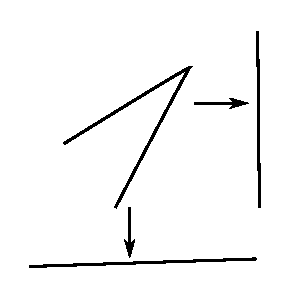
\includegraphics{figure/fig7.eps}
\end{figure}
\noindent
cannot be triangulated.
\end{ex}

\begin{ex}\label{chap1-ex2.2.10}
Let $\mathscr{P}$ be a presentation of a polyhedron $P$ in $V$. $\varphi:V\to W$ be a linear map, then $\varphi(\mathscr{P})=\{\varphi(C)|C\in\mathscr{P}\}$ is a presentation of $\varphi(P)$.
\end{ex}

\begin{ex}\label{chap1-ex2.2.11}
Let $f:P\to Q$ be a polyhedral map, and $X$ a subpolyhedron of $P$. Then $\dim f(X)\leq \dim X$.
\end{ex}

\begin{ex}\label{chap1-ex2.2.12}
If $f:P\to Q$ is a polyhedral map $Y$ is a subpolyhedron of $Q$, $f^{-1}(Y)$ is a subpolyhedron of $X$.
\end{ex}

Next, one can discuss abstract simplicial complexes, their geometric realizations etc. We do not need them until the last chapter. The reader is referred to Pontryagin's little book mentioned in the first chapter for these things.




